%%
% 结论
% 结论是毕业论文的总结,是整篇论文的归宿,应精炼、准确、完整。结论应着重阐述自己的创造性成果及其在本研究领域中的意义、作用,还可进一步提出需要讨论的问题和建议。
% modifyer: 黄俊杰(huangjj27, 349373001dc@gmail.com)
% update date: 2017-04-13
%%

\chapter{试验结果}
在总图片数200张,其中包含斑马线的图片100张,不包含斑马线的图片100张。不包含斑马线的图片来自:无斑马线的街景、室内照片、建筑物、风景和一些随机图片。
\begin{table}[h] %voc table result
	\centering
		\begin{tabular}{*{4}{c}}
			\toprule
	 		Method & precision & recall \\
			\midrule
			双极系数 & 75.6 & 79 \\
		    Hough变换 & 88.3 & 80.6 \\
			支持向量机 & 86.4 & 93.7 \\
			加权判据 & 88 & 89.5 \\
			\bottomrule
		\end{tabular}
		\caption{实验对比表格}
\end{table}
\par
\begin{figure}[h]
    \centering
    \begin{subfigure}{.5\textwidth}
      \centering
      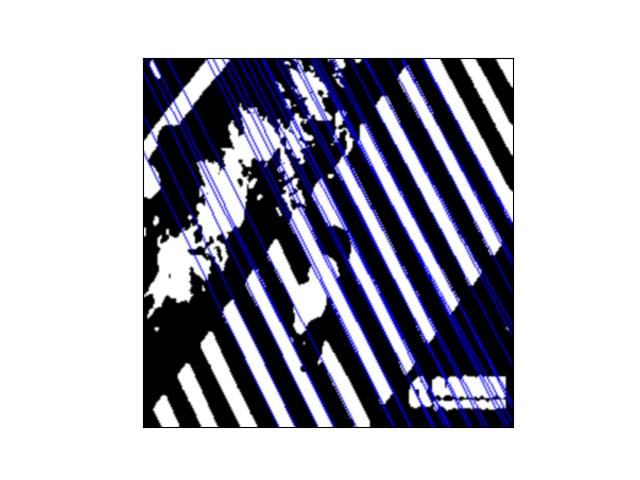
\includegraphics[width=\linewidth]{image/wrong1.png}
      \caption{颜色检测错误}
    \end{subfigure}%
    \begin{subfigure}{.5\textwidth}
      \centering
      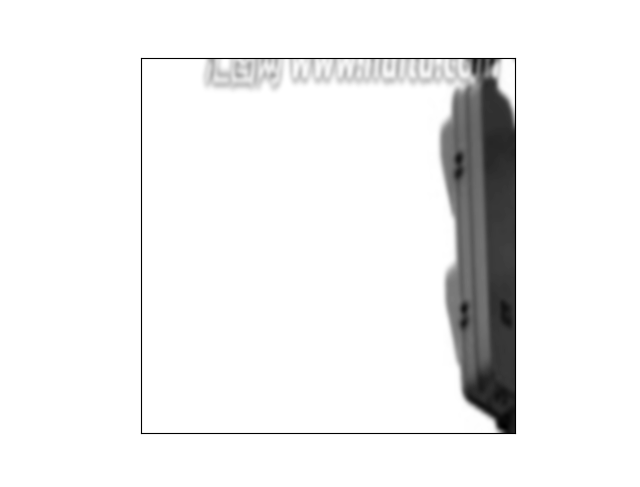
\includegraphics[width=\linewidth]{image/bipolar/90736.png}
      \caption{双极系数错误}
    \end{subfigure}
    \caption{典型情况错误分析}
\end{figure}
\par
已经观测到的错误原因如图5-1(a),Hough判据已经找出直线的情况下,由于斑马线恰好占据ROI的对角线,因此无法确认对应区域的颜色(黑色和白色几乎一样多)导致生成字符串中的一个B变为X。
另一种错误原因如图5-1(b),双极系数容易被黑白图片迷惑。

